%% fig_massgap.tex   (generated by make_round19.py; do not edit by hand)
%% The conjecture as a mass gap (thm:massgap): the real minimum k L_h(c), the integral minima above it with ||kc||_Z / k -> L_h(c), algebraic exactly when a minimum lies on the line; and the exact numbers of the Mumford square (ex:mumfordmass).
\documentclass[tikz,border=8pt]{standalone}
\usepackage{amsmath,amssymb}
\usetikzlibrary{arrows.meta,calc,decorations.pathreplacing}
%% palette.tex -- shared colour definitions for the figures
\definecolor{PInk}{RGB}{26,32,44}
\definecolor{PBlue}{RGB}{37,82,139}
\definecolor{PTeal}{RGB}{23,127,125}
\definecolor{POchre}{RGB}{193,138,44}
\definecolor{PClay}{RGB}{178,74,58}
\definecolor{PSlate}{RGB}{108,122,137}
\definecolor{PViolet}{RGB}{110,86,150}
\definecolor{WBlue}{RGB}{223,234,246}
\definecolor{WTeal}{RGB}{220,238,236}
\definecolor{WOchre}{RGB}{250,240,218}
\definecolor{WClay}{RGB}{247,229,224}
\definecolor{WSlate}{RGB}{238,241,244}
\definecolor{PMag}{RGB}{158,58,110}
\definecolor{PGrass}{RGB}{62,124,66}
\definecolor{PAmber}{RGB}{214,112,38}
\definecolor{PIndigo}{RGB}{58,64,140}
\definecolor{PRule}{RGB}{176,186,197}

%% shared macros so the standalone figures match the paper
\providecommand{\QQ}{\mathbb{Q}}
\providecommand{\ZZ}{\mathbb{Z}}
\providecommand{\RR}{\mathbb{R}}
\providecommand{\CC}{\mathbb{C}}
\providecommand{\PP}{\mathbb{P}}
\providecommand{\Kx}{K^{\times}}
\providecommand{\HW}{W}
\providecommand{\Nm}{\mathrm{N}}
\providecommand{\Hdg}{\mathrm{Hdg}}
\providecommand{\NS}{\mathrm{NS}}
\providecommand{\cA}{\mathcal{A}}
\providecommand{\cD}{\mathcal{D}}
\providecommand{\cF}{\mathcal{F}}
\providecommand{\cP}{\mathcal{P}}
\providecommand{\cO}{\mathcal{O}}
\providecommand{\cQ}{\mathcal{Q}}
\providecommand{\bbar}[1]{\overline{#1}}
\providecommand{\ch}{\operatorname{ch}}
\providecommand{\End}{\mathrm{End}}
\providecommand{\Ext}{\operatorname{Ext}}
\providecommand{\Supp}{\operatorname{Supp}}

\begin{document}
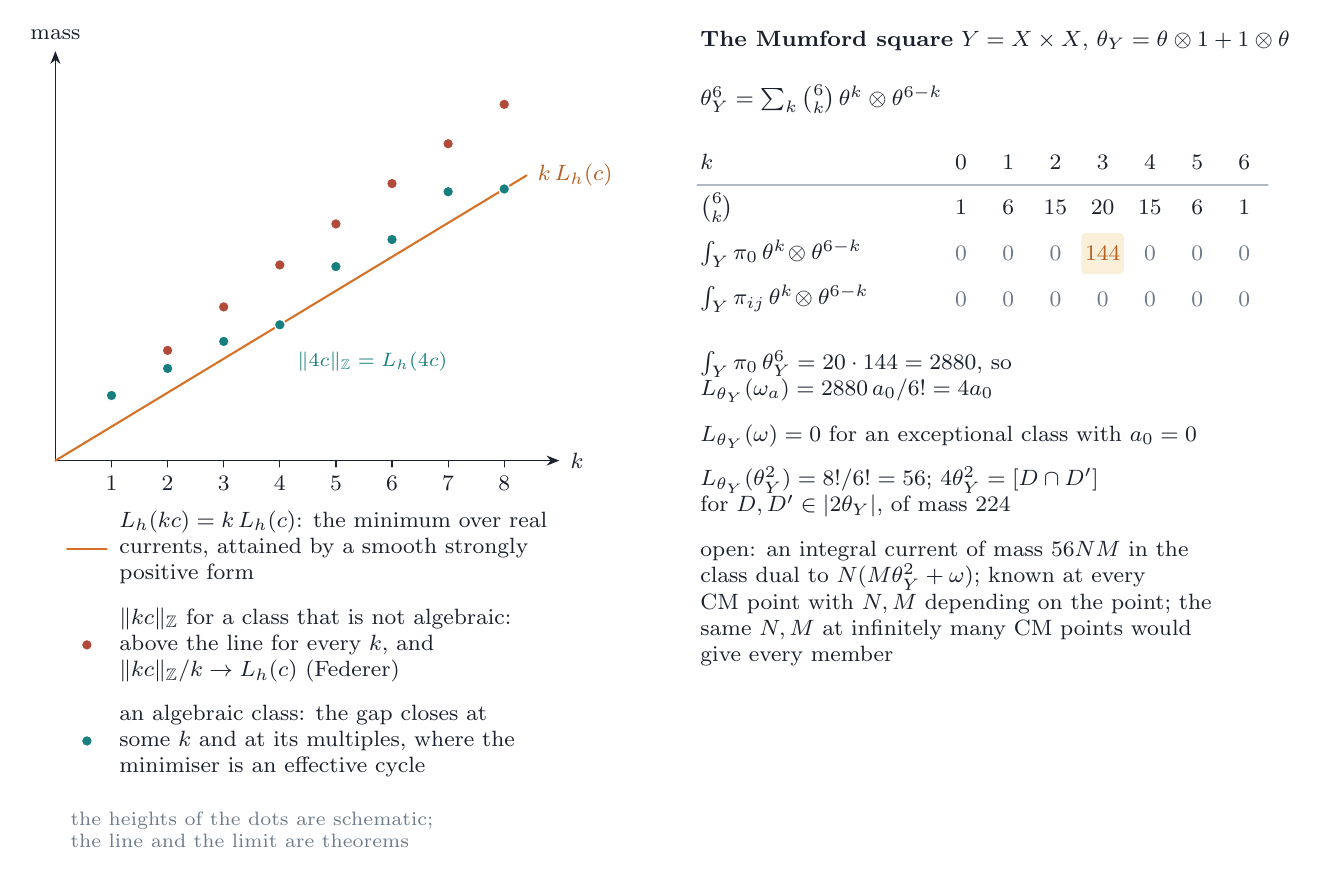
\begin{tikzpicture}[x=1cm,y=1cm,line join=round,line cap=round,
  font=\small,text=PInk,lbl/.style={inner sep=1pt}]
  \path[fill=WOchre,draw=none,rounded corners=1.5pt] (13.0300,2.3700) rectangle (13.5700,2.8900);
  \draw[PInk,line width=0.55pt,-{Stealth[length=4.6pt,width=3.6pt]}] (0.0000,0.0000) -- (6.4000,0.0000);
  \draw[PInk,line width=0.55pt,-{Stealth[length=4.6pt,width=3.6pt]}] (0.0000,0.0000) -- (0.0000,5.2000);
  \draw[PInk,line width=0.45pt] (0.7125,0.0000) -- (0.7125,-0.0800);
  \draw[PInk,line width=0.45pt] (1.4250,0.0000) -- (1.4250,-0.0800);
  \draw[PInk,line width=0.45pt] (2.1375,0.0000) -- (2.1375,-0.0800);
  \draw[PInk,line width=0.45pt] (2.8500,0.0000) -- (2.8500,-0.0800);
  \draw[PInk,line width=0.45pt] (3.5625,0.0000) -- (3.5625,-0.0800);
  \draw[PInk,line width=0.45pt] (4.2750,0.0000) -- (4.2750,-0.0800);
  \draw[PInk,line width=0.45pt] (4.9875,0.0000) -- (4.9875,-0.0800);
  \draw[PInk,line width=0.45pt] (5.7000,0.0000) -- (5.7000,-0.0800);
  \draw[PAmber,line width=0.75pt] (0.0000,0.0000) -- (5.9850,3.6225);
  \path[fill=PClay,draw=white,line width=0.50pt] (0.7125,0.8113) circle (2.00pt);
  \path[fill=PClay,draw=white,line width=0.50pt] (1.4250,1.3999) circle (2.00pt);
  \path[fill=PClay,draw=white,line width=0.50pt] (2.1375,1.9519) circle (2.00pt);
  \path[fill=PClay,draw=white,line width=0.50pt] (2.8500,2.4850) circle (2.00pt);
  \path[fill=PClay,draw=white,line width=0.50pt] (3.5625,3.0060) circle (2.00pt);
  \path[fill=PClay,draw=white,line width=0.50pt] (4.2750,3.5183) circle (2.00pt);
  \path[fill=PClay,draw=white,line width=0.50pt] (4.9875,4.0241) circle (2.00pt);
  \path[fill=PClay,draw=white,line width=0.50pt] (5.7000,4.5248) circle (2.00pt);
  \path[fill=PTeal,draw=white,line width=0.50pt] (0.7125,0.8273) circle (2.00pt);
  \path[fill=PTeal,draw=white,line width=0.50pt] (1.4250,1.1705) circle (2.00pt);
  \path[fill=PTeal,draw=white,line width=0.50pt] (2.1375,1.5138) circle (2.00pt);
  \path[fill=PTeal,draw=white,line width=0.50pt] (2.8500,1.7250) circle (2.00pt);
  \path[fill=PTeal,draw=white,line width=0.50pt] (3.5625,2.4642) circle (2.00pt);
  \path[fill=PTeal,draw=white,line width=0.50pt] (4.2750,2.8075) circle (2.00pt);
  \path[fill=PTeal,draw=white,line width=0.50pt] (4.9875,3.4148) circle (2.00pt);
  \path[fill=PTeal,draw=white,line width=0.50pt] (5.7000,3.4500) circle (2.00pt);
  \draw[PAmber,line width=0.75pt] (0.1500,-1.1200) -- (0.6500,-1.1200);
  \path[fill=PClay,draw=white,line width=0.50pt] (0.4000,-2.3400) circle (2.00pt);
  \path[fill=PTeal,draw=white,line width=0.50pt] (0.4000,-3.5600) circle (2.00pt);
  \draw[PRule,line width=0.45pt] (8.1500,3.5000) -- (15.4000,3.5000);
  \node[lbl,anchor=west,text=PInk,font=\footnotesize] at (6.5000,0.0000) {$k$};
  \node[lbl,anchor=south,text=PInk,font=\footnotesize] at (0.0000,5.3000) {mass};
  \node[lbl,anchor=north,text=PInk,font=\footnotesize] at (0.7125,-0.1600) {$1$};
  \node[lbl,anchor=north,text=PInk,font=\footnotesize] at (1.4250,-0.1600) {$2$};
  \node[lbl,anchor=north,text=PInk,font=\footnotesize] at (2.1375,-0.1600) {$3$};
  \node[lbl,anchor=north,text=PInk,font=\footnotesize] at (2.8500,-0.1600) {$4$};
  \node[lbl,anchor=north,text=PInk,font=\footnotesize] at (3.5625,-0.1600) {$5$};
  \node[lbl,anchor=north,text=PInk,font=\footnotesize] at (4.2750,-0.1600) {$6$};
  \node[lbl,anchor=north,text=PInk,font=\footnotesize] at (4.9875,-0.1600) {$7$};
  \node[lbl,anchor=north,text=PInk,font=\footnotesize] at (5.7000,-0.1600) {$8$};
  \node[lbl,anchor=west,text=PAmber!85!black,font=\footnotesize] at (6.0850,3.6225) {$k\,L_{h}(c)$};
  \node[lbl,anchor=west,text=PTeal,font=\scriptsize] at (3.0300,1.2598) {$\|4c\|_{\ZZ}=L_{h}(4c)$};
  \node[lbl,anchor=west,text=PInk,font=\footnotesize,align=left] at (0.7700,-1.1000) {$L_{h}(kc)=k\,L_{h}(c)$: the minimum over real\\currents, attained by a smooth strongly\\positive form};
  \node[lbl,anchor=west,text=PInk,font=\footnotesize,align=left] at (0.7700,-2.3400) {$\|kc\|_{\ZZ}$ for a class that is not algebraic:\\above the line for every $k$, and\\$\|kc\|_{\ZZ}/k\to L_{h}(c)$ (Federer)};
  \node[lbl,anchor=west,text=PInk,font=\footnotesize,align=left] at (0.7700,-3.5600) {an algebraic class: the gap closes at\\some $k$ and at its multiples, where the\\minimiser is an effective cycle};
  \node[lbl,anchor=west,text=PSlate,font=\scriptsize,align=left] at (0.1500,-4.6882) {the heights of the dots are schematic;\\the line and the limit are theorems};
  \node[lbl,anchor=west,text=PInk,font=\footnotesize] at (8.1500,5.3329) {\textbf{The Mumford square} $Y=X\times X$, $\theta_{Y}=\theta\otimes1+1\otimes\theta$};
  \node[lbl,anchor=west,text=PInk,font=\footnotesize] at (8.1500,4.5900) {$\theta_{Y}^{6}=\sum_{k}\binom6k\,\theta^{k}\otimes\theta^{6-k}$};
  \node[lbl,anchor=west,text=PInk,font=\footnotesize] at (8.1500,3.7900) {$k$};
  \node[lbl,anchor=west,text=PInk,font=\footnotesize] at (8.1500,3.2100) {$\binom6k$};
  \node[lbl,anchor=west,text=PInk,font=\footnotesize] at (8.1500,2.6300) {$\int_{Y}\pi_{0}\,\theta^{k}\!\otimes\theta^{6-k}$};
  \node[lbl,anchor=west,text=PInk,font=\footnotesize] at (8.1500,2.0500) {$\int_{Y}\pi_{ij}\,\theta^{k}\!\otimes\theta^{6-k}$};
  \node[lbl,text=PInk,font=\footnotesize] at (11.5000,3.7900) {$0$};
  \node[lbl,text=PInk,font=\footnotesize] at (11.5000,3.2100) {$1$};
  \node[lbl,text=PSlate,font=\footnotesize] at (11.5000,2.6300) {$0$};
  \node[lbl,text=PSlate,font=\footnotesize] at (11.5000,2.0500) {$0$};
  \node[lbl,text=PInk,font=\footnotesize] at (12.1000,3.7900) {$1$};
  \node[lbl,text=PInk,font=\footnotesize] at (12.1000,3.2100) {$6$};
  \node[lbl,text=PSlate,font=\footnotesize] at (12.1000,2.6300) {$0$};
  \node[lbl,text=PSlate,font=\footnotesize] at (12.1000,2.0500) {$0$};
  \node[lbl,text=PInk,font=\footnotesize] at (12.7000,3.7900) {$2$};
  \node[lbl,text=PInk,font=\footnotesize] at (12.7000,3.2100) {$15$};
  \node[lbl,text=PSlate,font=\footnotesize] at (12.7000,2.6300) {$0$};
  \node[lbl,text=PSlate,font=\footnotesize] at (12.7000,2.0500) {$0$};
  \node[lbl,text=PInk,font=\footnotesize] at (13.3000,3.7900) {$3$};
  \node[lbl,text=PInk,font=\footnotesize] at (13.3000,3.2100) {$20$};
  \node[lbl,text=PAmber!85!black,font=\footnotesize] at (13.3000,2.6300) {$144$};
  \node[lbl,text=PSlate,font=\footnotesize] at (13.3000,2.0500) {$0$};
  \node[lbl,text=PInk,font=\footnotesize] at (13.9000,3.7900) {$4$};
  \node[lbl,text=PInk,font=\footnotesize] at (13.9000,3.2100) {$15$};
  \node[lbl,text=PSlate,font=\footnotesize] at (13.9000,2.6300) {$0$};
  \node[lbl,text=PSlate,font=\footnotesize] at (13.9000,2.0500) {$0$};
  \node[lbl,text=PInk,font=\footnotesize] at (14.5000,3.7900) {$5$};
  \node[lbl,text=PInk,font=\footnotesize] at (14.5000,3.2100) {$6$};
  \node[lbl,text=PSlate,font=\footnotesize] at (14.5000,2.6300) {$0$};
  \node[lbl,text=PSlate,font=\footnotesize] at (14.5000,2.0500) {$0$};
  \node[lbl,text=PInk,font=\footnotesize] at (15.1000,3.7900) {$6$};
  \node[lbl,text=PInk,font=\footnotesize] at (15.1000,3.2100) {$1$};
  \node[lbl,text=PSlate,font=\footnotesize] at (15.1000,2.6300) {$0$};
  \node[lbl,text=PSlate,font=\footnotesize] at (15.1000,2.0500) {$0$};
  \node[lbl,anchor=west,text=PInk,font=\footnotesize,align=left] at (8.1500,1.0648) {$\int_{Y}\pi_{0}\,\theta_{Y}^{6}=20\cdot144=2880$, so\\$L_{\theta_{Y}}(\omega_{a})=2880\,a_{0}/6!=4a_{0}$};
  \node[lbl,anchor=west,text=PInk,font=\footnotesize,align=left] at (8.1500,0.3039) {$L_{\theta_{Y}}(\omega)=0$ for an exceptional class with $a_{0}=0$};
  \node[lbl,anchor=west,text=PInk,font=\footnotesize,align=left] at (8.1500,-0.4018) {$L_{\theta_{Y}}(\theta_{Y}^{2})=8!/6!=56$; $4\theta_{Y}^{2}=[D\cap D']$\\for $D,D'\in|2\theta_{Y}|$, of mass $224$};
  \node[lbl,anchor=west,text=PInk,font=\footnotesize,align=left] at (8.1500,-1.8149) {open: an integral current of mass $56NM$ in the\\class dual to $N(M\theta_{Y}^{2}+\omega)$; known at every\\CM point with $N,M$ depending on the point; the\\same $N,M$ at infinitely many CM points would\\give every member};
\end{tikzpicture}
\end{document}
